\part{Week 5}
\chapter{Entropy and information}
We know that \textit{entropy} measures uncertainity of state of a physical system. We'll look into it's definitions and properties deeply both in classical and quantum information theory.

\section{Shannon entropy}
It's the key concept of classical information theory. It can be viewed in two complementary views, first, suppose we have a random variable $X$, how much information we \textit{gain} on average if we know the value of $X$. Second, it's the measure of \textit{uncertainity} before we know the value of $X$.

Information content of a random variable doesn't depend on labels. For example, a random variaible giving `heads' and `tails' with probability $1/4$ and $3/4$ contains same information as a random variable giving `$0$' and `$1$' with probability $1/4$ and $3/4$ respectively. Thus, entropy also doesn't depend on labels. \textit{Shannon entropy} associated with a probability distribution $p_1,\dots,p_n$ is given by
\begin{equation}
    H(X) \equiv H(p_1,\dots,p_n) \equiv -\sum_x p_x\log p_x
\end{equation}
Note that by $\log$ we mean base $2$, by $\ln$ we mean base $e$. Since a never occuring event with probability $p_i=0$ should never affect entropy, thus we agree that $0\log 0=0$ even though we mean $\lim_{x\rightarrow0} x\log x = 0$. There's a nice reason why entropy is defined this way. We have to \textit{quantify the resources needed to store information}. Let's suppose a source producing symbols $X_1,X_2,\dots$ of independent \textit{identically} distributed random variables, minimal amount of resources required to store the information produced by source such that it can be reconstructed turns out to be just entropy i.e $H(X)\equiv H(X_1) \equiv H(X_2) = \dots$, this result is known as \textit{Shannon's noiseless coding theorem}.

I suggest looking at an example to understand this. Suppose our source produces $1$, $2$, $3$, $4$ which are symbols but with probability $1/2$, $1/4$, $1/8$ and $1/8$ respectively. We don't need two bits to store output of each use of source. We can compress this usage, by representing $1$ as $0$, $2$ as $10$, $3$ as $110$ and $4$ as $111$, with this we can reconstruct the message, for eg. $11010111$ as $324$ too. We need on an average $\frac{1}{2}\cdot 1 + \frac{1}{4}\cdot 2 + \frac{1}{8}\cdot 3 + \frac{1}{8}\cdot 3 = 7/4$ bits only! It also turns out that this is just the entropy of the source $H(X) = -1/2\log(1/2) - 1/4\log(1/4) - 1/8\log(1/8) - 1/8\log(1/8) = 7/4$. It's also true that average information gained by an event out of a probability distribution $p_1,\dots,p_n$ is $k\sum_ip_i\log p_i$ for some constant $k$.

\section{Basic properties of entropy}
\subsection{The binary entropy}
The entropy of a two-outcome random variable is so special that we name it as \textit{binary entropy}
\begin{equation}
    H_{\text{bin}}(X) \equiv -p\log p - (1-p)\log (1-p)
\end{equation}
where $p$ and $1-p$ are probabilities of outcome. It's graph is shown in figure  \ref{fig:binary-entropy} 
\begin{figure}
    \centering
    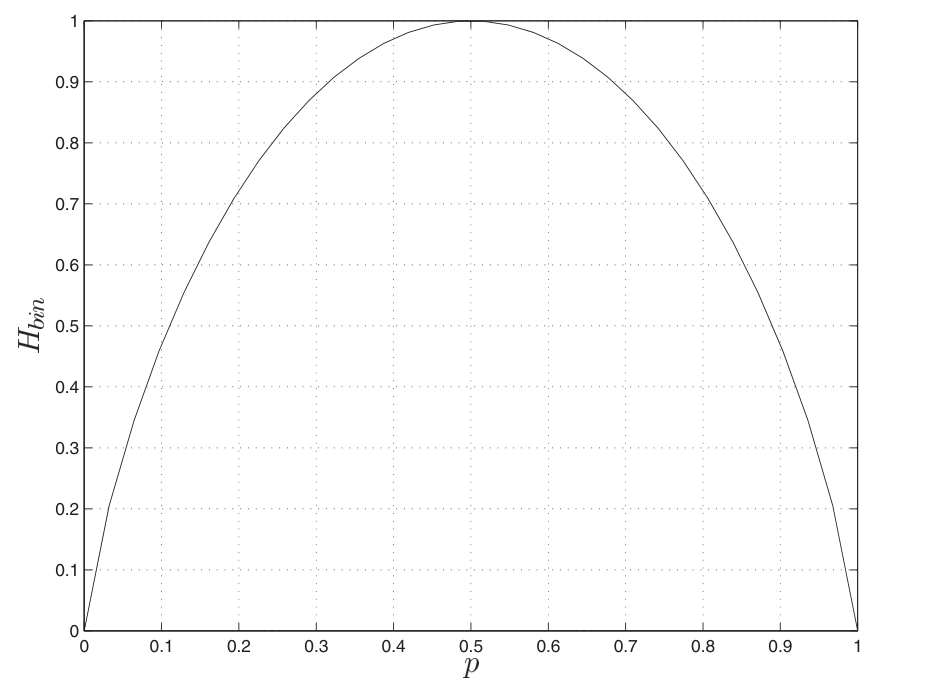
\includegraphics[width=0.65\textwidth]{images/binary_entropy.png}
    \caption{Binary entropy function $H(p)$}
    \label{fig:binary-entropy}
\end{figure}

A really good intuition comes when we consider this example of Alice having two biased coins one from US and another from Australia. Suppose the US coin gives head with probability $p_U$ and the Australian coin with probability $p_A$ and Alice flips one of those coins with probability $q$ for US coin and $1-q$ for Australian coin and she tells final `head' or `tail' to Bob. The information Bob gets is atleast the average information he gets from flipping one coin. Hence
\begin{equation}
    H(qp_U + (1-p)p_A) \geq qH(p_U) + (1-q)H(p_A)
\end{equation}
It's greater because Bob gets \textit{more} information about the country sometimes. For eg. if $p_U=0.1$ and $p_A=0.9$ and Alice says head, Bob would understand that it's more probable to be an aussie coin. This leads us into a very important property of entropy, \textit{concavity}. Which can be seen in binary case in the figure \ref{fig:binary-entropy}.

\subsection{The relative entropy}
The \textit{relative entropy} is useful entropy-like measure describing closeness of two probability distributions $p(x)$ and $q(x)$ over the same index set $x$, defined by
\begin{equation}
    H(p(x) \parallel q(x)) \equiv \sum_x p(x)\log \frac{p(x)}{q(x)} \equiv -H(X)-\sum_x p(x)\log q(x)
\end{equation}
The following theorem motivates us to understand it as a distance measure
\begin{theorem}[\textbf{Non-negativity of relative entropy}]
    The relative entropy is non-negative, $H(p(x) \parallel q(x)) \geq 0$ with equality if and only if $p(x)=q(x)$ for all $x$.
    \label{thm:non-negativity-of-rel-entropy}
\end{theorem}
The proof is simple using the definition of relative entropy and $\log x \ln{2} \leq x-1$ with equality only when $x=1$. Relative entropy itself is not very useful but used to study entropy, for example let $q(x)$ be uniform probability distribution over index set $X$ of size $d$ then for a probability distribution $p(x)$ over $X$, we have
\begin{equation}
    H(p(x)\parallel q(x)) = H(p(x)\parallel 1/d) = -H(X) - \sum_x p(x) \log (1/d) = \log d - H(X)
\end{equation}
and hence by theorem \ref{thm:non-negativity-of-rel-entropy} we have $\log d - H(X) \geq 0$ thus $H(X) \leq \log d$, a nice property hence a theorem!
\begin{theorem}
    Suppose $X$ is a random variable with $d$ outcomes. Then $H(X) \leq \log d$, with equality if and only if $X$ is uniformly distributed over those $d$ outcomes.
\end{theorem}

\subsection{Conditional entropy and mutual information}
For two random variables $X$, $Y$ we'll try to understand how information of $X$ is related to that of $Y$. First we define \textit{joint entropy} of $X$ and $Y$ as
\begin{equation}
    H(X, Y) \equiv -\sum_{x, y} p(x, y)\log p(x, y)
\end{equation}
The \textit{entropy of $X$ conditional on knowing $Y$} is similar to that in probability, it's the uncertainity that we have in the value of $X$ given that we know the value of $Y$. It's defined by
\begin{equation}
    H(X | Y) \equiv H(X,Y) - H(Y)
\end{equation}

A second quantity \textit{mutual information content of $X$ and $Y$} measures how much information $X$ and $Y$ have in common. It's very similar to intersection, given we take $H(X,Y)$ as information content of both $X$ and $Y$ which is counted twice. Thus, mutual information content is
\begin{equation}
    H(X:Y) = H(X) + H(Y) - H(X, Y)
\end{equation}
The relation $H(X:Y) = H(X) - H(X|Y)$ also comes in handy. Let's see some more simple relationships between different entropies.

\begin{ntheorem}[\textbf{Basic properties of Shannon entropy}]
    \begin{enumerate}
        \item $H(X, Y) = H(Y, X), H(X:Y) = H(Y:X)$
        \item $H(Y|X) \geq 0$ and thus $H(X:Y)\leq H(Y)$ with equality if and only if $Y$ is a function of $X$, $Y=f(X)$.
        \item $H(X) \leq H(X,Y)$ with equality if and only if $Y$ is a function of $X$.
        \item \textbf{Subadditivity:} $H(X, Y) \leq H(X) + H(Y)$ with equality if and only if $X$ and $Y$ are independent variables.
        \item $H(Y|X) \leq H(Y)$ and thus $H(X:Y) \geq 0$ with equality in each if and only if $X$ and $Y$ are independent distributions.
        \item \textbf{Strong subadditivity:} $H(X,Y,Z) + H(Y) \leq H(X,Y) + H(Y, Z)$, with equality if and only if $Z\rightarrow Y\rightarrow X$ forms a markov chain.
        \item \textbf{Conditioning reduces entropy:} $H(X|Y,Z) \leq H(X|Y)$.
    \end{enumerate}
\end{ntheorem}
All this can be easily understood by a Venn diagram for entropy.
\begin{figure}[H]
    \centering
    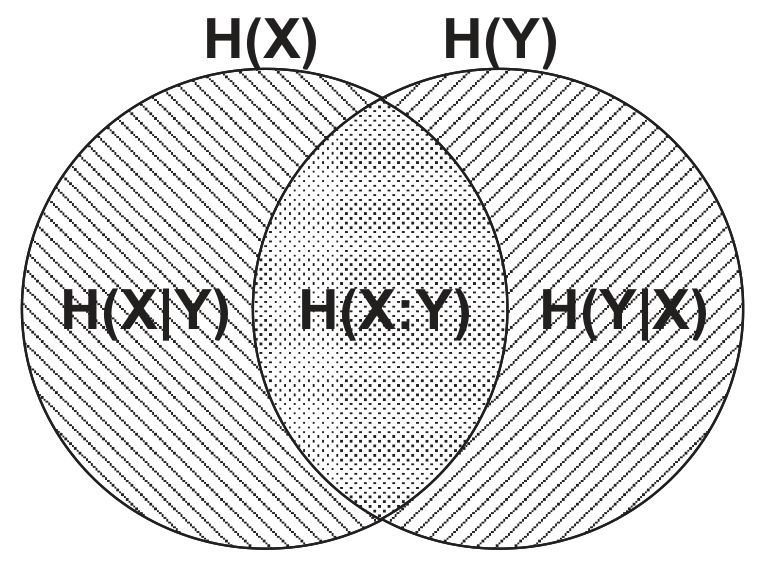
\includegraphics[width=0.45\textwidth]{images/venn_entropy.png}
    \caption{Relationships between different entropies}
    \label{fig:venn-entropy}
\end{figure}
Let's finally consider a simple and useful chaining rule for conditional entropies.
\begin{theorem}
    Let $X_1,\dots,X_n$ and $Y$ be any set of random variables. Then
    \begin{equation}
        H(X_1,\dots,X_n|Y) = \sum_{i=1}^n H(X_i|Y,X_1,\dots,X_{i-1})
    \end{equation}
\end{theorem}
\begin{proof}
    Use induction with base case $n=2$.
\end{proof}

\subsection{The data processing inequality}
This states that information from the output of a source can only \textit{decrease with time}; once information is lost, it's gone forever. The intuitive notion of \textit{information processing} is captured by \textit{Markov chanis} of random variables. A Markov chain is a sequence $X_1\rightarrow X_2 \rightarrow \cdots$ such that $X_{n+1}$ is independent of $X_1, X_2, \dots, X_{n-1}$ if $X_n$ is known. In other words
\begin{equation}
    p(X_{n+1}=x_{n+1} | X_n = x_n, %{X_{n-1} = x_{n-1}},
    \dots, X_1 = x_1) = p(X_{n+1}=x_{n+1} | X_n = x_n)
\end{equation}

\begin{theorem}
    Suppose $X\rightarrow Y \rightarrow Z$ is a Markov chain. Then
    \begin{equation}
        H(X) \geq H(X:Y) \geq H(X:Z).
    \end{equation}
    Moreover, this first inequality becomes equal if and only if, given $Y$, it's possible to reconstruct $X$.
\end{theorem}
This theorem is intuitive, as it says that if there's some noise introduced in $X$ (which leads to Markov chain $X\rightarrow Y$) then the mutual information between $X$ and $Y$ (which is what we want) is irretrievably lost, since it's not possible to reconstruct $X$ from $Y$ (noise).

If $X\rightarrow Y \rightarrow Z$ is a Markov chain, then so is $Z\rightarrow Y \rightarrow X$\footnote{Can be proved by using $P(X|Y)=P(X,Y)/P(Y)$}. Thus with above conditions, we see that
\begin{equation}
    H(Z:Y) \geq H(Z:X)
\end{equation}
This thing is also known as \textit{data pipelining inequality} i.e any information $Z$ shares with $X$ is also shared by $Y$. The information is \textit{pipelined} from $X$ to $Y$ to $Z$.

\section{Von Neumann entropy}
Shannon entropy is for classical probability distributions, Von Neumann defined this notion of \textit{entropy} for quantum state with density operator $\rho$ as 
\begin{equation}
    S(\rho) \equiv -\tr{\rho \log{\rho}}
\end{equation}
where $\log$ still means base $2$ and $0\log 0 \equiv 0$. This can be simplified if we know eigenvalues $\lambda_x$ of $\rho$ as
\begin{equation}
    S(\rho) \equiv -\sum_x \lambda_x \log{\lambda_x}
\end{equation}
This is very useful for calculations. We will refer \textit{entropy} to either Shannon or Von Neumann entropy based on context.

\subsection{Quantum relative entropy}
Similar to Shannon entropy, \textit{relative entropy} between two state $\rho$ and $\sigma$ is defined by
\begin{equation}
    S(\rho \parallel \sigma) \equiv \tr{\rho \log{\rho}} - \tr{\rho \log{\sigma}}
\end{equation}
as in classical case, this can sometimes shoot upto infinity. Particularly, relative entropy is defined to be $+\infty$ if the kernel of $\sigma$ (vector space spanned by eigenvectors of $\sigma$ with eigenvalue $0$) has non-trivial intersection with the support of $\rho$ (vector space spanned by eigenvectors of $\rho$ with non-zero eigenvalues). A familiar inequality as a theorem is given.
\begin{theorem}[\textbf{Klein's inequality}]
    The quantum relative entroy is non-negative. i.e
    \begin{equation}
        S(\rho \parallel \sigma) \geq 0,
    \end{equation}
    with equality if and only if $\rho=\sigma$.
\end{theorem}

\subsection{Basic properties of entropy}
These are few interesting properties of von Neumann entropy:
\begin{ntheorem}[\textbf{Basic properties of von Neumann entropy}]
    \begin{enumerate}
        \item The entropy is non-negative. The entropy is zero if and only if the state is pure.
        \item In a $d$-dimensional Hilbert space, entropy is atmost $\log{d}$. It's equal if and only if the system is completely mixed state $I/d$.
        \item If a composite system $AB$ is pure, then $S(A)=S(B)$.
        \item Suppose $p_i$ are probabilities and $\rho_i$ have support on orthogonal subspaces. Then 
        \begin{equation}
            S\left( \sum_i p_i\rho_i \right) = H(p_i) + \sum_i p_iS(\rho_i)
        \end{equation}
        \item \textbf{Joint entropy theorem:} Suppose $p_i$ are probabilities and $\ket{i}$ are orthogonal states for a system $A$, and $\rho_i$ is any set of density operators for another system, $B$. Then
        \begin{equation}
            S\left( \sum_i p_i\op{i} \otimes \rho_i \right) = H(p_i) + \sum_i p_iS(\rho_i).
        \end{equation}
    \end{enumerate}
\end{ntheorem}

Again similarly, the \textit{joint entropy} $S(A, B)$ for a composite system of two components $A$ and $B$ is defined obviously as $S(A, B) \equiv -\tr{\rho^{AB}\log{\rho^{AB}}}$, we also define conditional entropy and mutual information as
\begin{align}
    S(A|B) &= S(A,B) - S(B) \\
    S(A:B) &= S(A) + S(B) - S(A, B) \\
    &= S(A)-S(A|B) = S(B) - S(B|A). 
\end{align}

But there are some properties which aren't carried over from Shannon to von Neumann entropy. One such is $H(X,Y)\geq H(X)$ which is intuitive since we have more information if we know about $X$ and $Y$ compared to if we only know about $X$. But this isn't true for von Neumann entropy, consider a system $AB$ of two qubits in entangled state $(\ket{00}+\ket{11})/\sqrt{2}$. Since this is pure, $S(A, B)=0$. But it's component $A$ is $I/2$, and has entropy $1$ defying what we've seen above. Another way of seeing this is $S(B|A) = S(A, B) - S(A)$ is negative.

\subsection{Measurements and entropy}
We'll try to understand how measurements change the entropy of a system, if they do. This change ofcourse depends on the type of measurement we make. Suppose we do a projective measurement on system $\rho$ described by projectors $P_i$, the state of the system is
\begin{equation}
    \rho' = \sum_i P_i\rho P_i
\end{equation}
The following theorem shows the entropy never decreases
\begin{theorem}[\textbf{Projective measurements increase entropy}]
    Suppose $P_i$ is a complete set of orthogonal projectors and $\rho$ is a density operator. Then the entropy of the state $\rho' \equiv \sum_iP_i\rho P_i$ of the system after measurement is atleast as great as the original entropy,
    \begin{equation}
        S(\rho') \geq S(\rho)
    \end{equation}
    with equality if and only if $\rho' = \rho$.
\end{theorem}

\subsection{Subadditivity}
If two system $A$ and $B$ have a joint state $\rho^{AB}$. Then the joint entropy for the two systems satisfy
\begin{align}
    S(A,B) &\leq S(A) + S(B) \\
    S(A,B) &\geq |S(A) - S(B)|
\end{align}
The first relation is known as \textit{subadditivity} inequality\footnote{This can be proved simply using Klein's inequality.} for von Neumann entropy, with equality if and only if $A$ and $B$ are correlated, i.e $\rho^{AB}=\rho^A\otimes \rho^B$. Second one is known as \textit{triangle} inequality or \textit{Araki-Lieb} inequality. It's the quantum analogue of $H(X,Y)\geq H(X)$.

\subsection{Concavity of the entropy}
The entropy is a \textit{concave} function in its inputs. That is, given the probabilities $p_i$, and corresponding density operators $\rho_i$, entropy satisfies the inequality\footnote{To prove this we introduce an auxillary system $B$.}
\begin{equation}
    S\left( \sum_i p_i\rho_i \right) \geq \sum_i p_i S(\rho_i).
\end{equation}
A good intuition is that $\sum_ip_i\rho_i$ expresses a quantum state which is in an uncertain state $\rho_i$ with probability $p_i$, this uncertainity of index $i$ of state adds to the average uncertainity we have of each state $\rho_i$ which is $\sum_i p_iS(\rho_i)$. Equality holds if and only if all the states $\rho_i$ for which $p_i>0$ are identical; i.e, entropy is strictly concave in its inputs!

\subsection{The entropy of a mixture of quantum states}
The flip side of concavity is that it provides an upper bound of entropy of a mixture of quantum states too. It's shown by the following theorem.
\begin{theorem}
    Suppose $\rho=\sum_ip_i\rho_i$, where $p_i$ are some set of probabilities, and $\rho_i$ are density operators. Then
    \begin{equation}
        S(\rho) \leq \sum_i p_iS(\rho_i) + H(p_i),
    \end{equation}
    with equality if and only if the states $\rho_i$ have support on orthogonal subspaces.
\end{theorem}
This along with concavity completes our bound on entropy of a mixture of quantum states,
\begin{equation}
    \sum_i p_iS(\rho_i) \leq S\left( \sum_ip_i\rho_i \right) \leq \sum_i p_iS(\rho_i) + H(p_i).
\end{equation}
The intuition for this comes from the fact that we know too much information if we know on average about $\rho_i$ and $p_i$ also.

\section{Strong subadditivity}
This is an extension of subadditivity and triangle inequalities to three systems. The inequality states that for three quantum systems $A$, $B$, $C$,
\begin{equation}
    S(A, B, C) + S(B) \leq S(A, B) + S(B, C)
\end{equation}
\subsection{Proving strong subadditivity}
The proof is based on an important result, the \textit{Lieb's theorem}. For which, let's define few things. A function $f(A, B)$ which is a real-valued function of two matrices, is said to be \textit{jointly concave} in $A$, $B$ if for all $0\leq \lambda \leq 1$,
\begin{equation}
    f(\lambda A_1 + (1-\lambda)A_2, \lambda B_1 + (1-\lambda)B_2) \geq \lambda f(A_1, B_1) + (1-\lambda)f(A_2, B_2).
\end{equation}
Let's state Lieb's theorem now,
\begin{theorem}[\textbf{Lieb's theorem}]
    Let $X$ be a matrix, and $0\leq t \leq 1$. Then the function
    \begin{equation}
        f(A, B) \equiv \tr{X^\dag A^tXB^{1-t}}
    \end{equation}
    is jointly concave in positive matrices $A$ and $B$.
\end{theorem}
This theorem implies another theorem, convexity of the relative entropy.
\begin{theorem}[\textbf{Convexity of the relative entropy}]
    The relative entropy $S(\rho \parallel \sigma)$ is jointly convex in its arguments.
\end{theorem}
\begin{corollary}[\textbf{Concavity of the quantum conditional entropy}]
    Let $AB$ be a composite quantum system with components $A$ and $B$. Then the conditional entropy $S(A|B)$ is concave in the state $\rho^{AB}$ of $AB$.
\end{corollary}
This finally leads us to strong subadditivity.
\begin{theorem}
    For any trio of quantum systems $A$, $B$, $C$ the inequalities
    \begin{align}
        S(A)+S(B) &\leq S(A,C) + S(B,C) \\
        S(A,B,C) + S(B) &\leq S(A,B) + S(B,C)
    \end{align}
    hold.
\end{theorem}

\subsection{Elementary applications of strong subadditivity}
Strong subadditivity and related results have many useful applications in quantum information theory. Take the inequality $S(A)+S(B)\leq S(A,C)+S(B,C)$ which is true, it also holds for Shannon entropy too, but for different reasons. For practical applications strong subadditivity is most easily applied as a rephrasing in terms of conditional and mutual entropies. Here are three major reformulations
\begin{ntheorem}[\textbf{Reformulations of strong subadditivity}]
    \begin{enumerate}
        \item \textbf{Conditioning reduces entropy:} Suppose $ABC$ is a composite system. Then $S(A|B,C)\leq S(A|B)$.
        \item \textbf{Discarding quantum systems never increases mutual information:} Suppose $ABC$ is a composite quantum system. Then $S(A:B) \leq S(A:B,C)$.
        \item \textbf{Quantum operations never increase mutual information:} Suppose $AB$ be a composite system and $\mathcal{E}$ is a trace preserving quantum operation on $B$. Let $S(A:B)$ be before operation, $S(A':B')$ be after operation, then $S(A':B') \leq S(A:B)$.
    \end{enumerate}
\end{ntheorem}
We saw before that Shannon mutual information is not subadditive, thus quantum mutual information isn't subadditive either. But it turns out that conditional entropy is subadditive, i.e
\begin{equation}
    S(A_1, A_2|B_1, B_2) \leq S(A_1|B_1) + S(A_2|B_2)
\end{equation}
What's more, it's subadditive in the first and second entries.
\begin{theorem}[\textbf{Subadditivity of conditional entropy}]
    Let $ABCD$ be a composite of four systems. Then the conditonal entropy is jointy subadditive in the first two entries:
    \begin{equation}
        S(A,B|C,D) \leq S(A|C) + S(B|D)
    \end{equation}
    Let $ABC$ be a composite of three quantum systems. Then conditional entropy is subadditive in each of first two entries:
    \begin{align}
        S(A,B|C) &\leq S(A|C) + S(B|C) \\
        S(A|B, C) &\leq S(A|B) + S(A|C)
    \end{align}
\end{theorem}
We got introduced to relative entropy like a measure between density operators. It seems intuitive that this relative entropy decreases when we ignore a part of system is ignored, i.e it makes it harder to distinguish two states of that system and thus decrease any reasonable measure of distance between them. This following theorem states it:
\begin{theorem}
    Let $\rho^{AB}$ and $\sigma^{AB}$ be any two density matrices of a composite system $AB$. Then
    \begin{equation}
        S(\rho^A \parallel \rho^A) \leq S(\rho^{AB} \parallel \rho^{AB}).
    \end{equation}
\end{theorem}